% Chapter Template

\chapter{Related Work} % Main chapter title

\label{Chapter5} % Change X to a consecutive number; for referencing this chapter elsewhere, use \ref{ChapterX}

\lhead{Chapter 5. \emph{Related Work}} % Change X to a consecutive
% number; this is for the header on each page - perhaps a shortened title

\section{The Attributed Graph Grammar System}

AGG is a general development environment for algebraic graph
transformation systems. AGG is provided with a graphical editor for creating
and modifying graphs. The editor provides a graphical user-interface with
several visual editors for applying the principles of graph transformation. It
also has an interpreter and a set of validation tools. AGG is ongoing research
activity of the graph grammar group at TU Berlin. The work on AGG started in 1997.

\subsection{Graphical Editor}
The graphical editor of AGG, represented in
figure~\ref{fig:AGGScreen}, has several functions to help the user to define
model transformations. In the top left corner of the graphical user-interface
is a tree based editor for defining rules and grammar. This tree based editor
also contains the type graphs and the host graphs. Where the host graph
represents some input model for a model transformation.

Each application rule has two visual editors, representing the left
(LHS) and the right hand side (RHS), or the pattern and the replacement graph.
In the tree based editor containing rules and grammars it is possible to give
rules application conditions. This is convenient if the user wants to have
constrains for the pattern or the replacement graph.

In the tree based visual editor it is also possible to define host
graphs and type graphs. Type graphs is described more in depths in the next
section, but roughly said, the type graph defines elements that can be used in
the host graph. Type graphs defines the abstract models for the host graph and
is similar to how Ecore defines metamodels  for EMF and the Meta Object
Facility (MOF)\cite{MOF}, that is a language for defining abstract syntax of
modeling languages. The users can now create instances from these type graphs.
These instances represents the host graphs and corresponds to its concurrent
type graph.

For the application rules, the user can extend the attributes with Java
expressions. This means that the users can use Java primitives such as strings,
integers or float numbers to form the pattern graph or the left hand side of
the rule. The user cannot bind attributes that is not initialised in the type graph.

In figure~\ref{fig:AGGScreen} there are some node elements and association
elements to the right side of the figure. These are meta elements that are
initialized in the type graph. These meta elements are used to create the host
graph, the different transformation rules and application conditions. The host
graph is not consistent with the type graph, since these meta elements are
initialized in the type graph. Its worth mentioning that both the
node elements and association elements in the figure has been scaled up for the
purpose of this paper.

\begin{figure}[H]
	\centering
	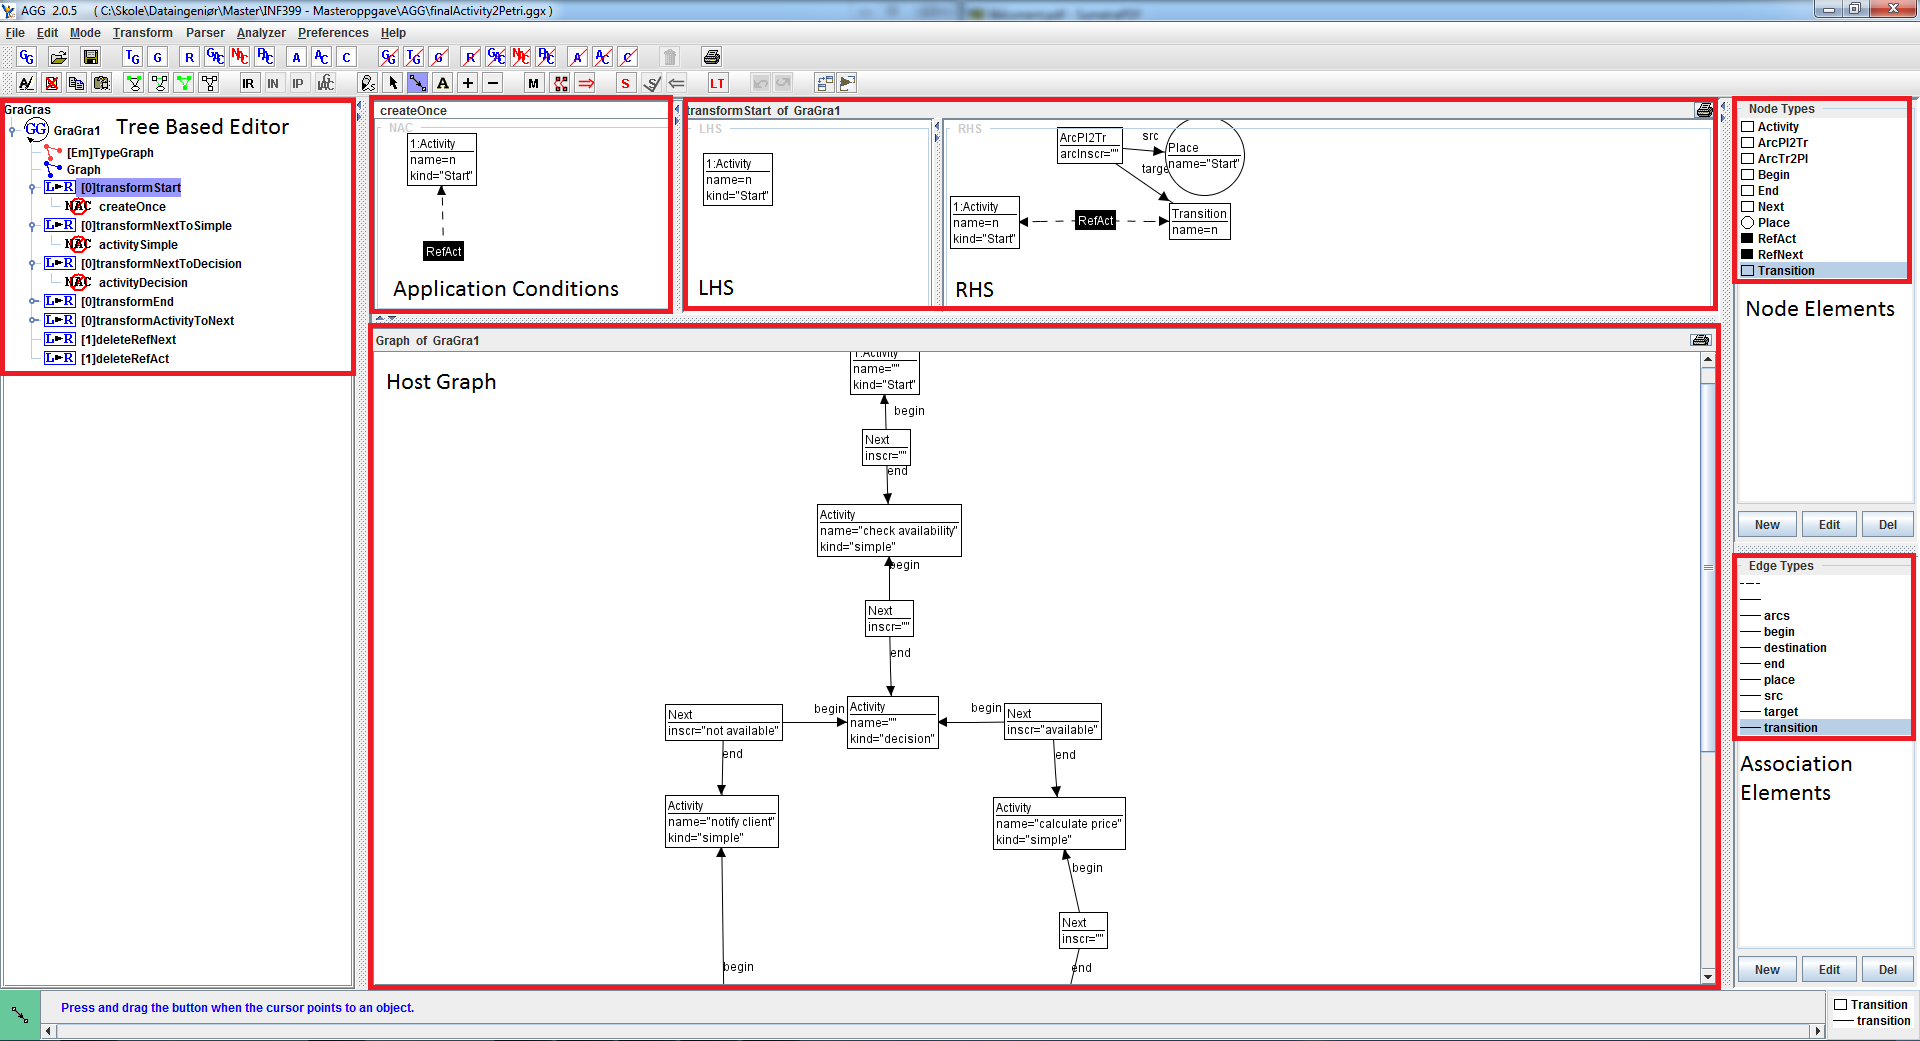
\includegraphics[scale=0.3]{figures/AGGscreen.png}
	\caption[Graphical Editor for AGG]
	{A model transformation for the AGG Editor.}
	\label{fig:AGGScreen}
\end{figure}

\subsection{Defining Metamodels}

Before the host graphs can be created, we have to initialise the AGG
tool with the metamodels. In AGG both the source and the target metamodel are
defined in a common type graph. This type graph represents the abstract syntax
for the host graph. If we want to prepare an AGG graph for a transformation, we
create a single type graph with references between elements of both source and
target metamodel. This way, when the application rules is executed, we can
choose to keep both the source graph and the references between these elements.
The references and source graph can be deleted through a cycle of transformation rules.

\begin{figure}[H]
	\centering
	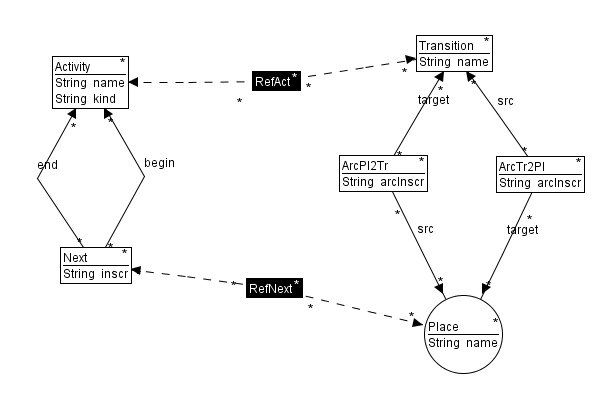
\includegraphics[scale=0.7]{figures/AggTypeGraph.png}
	\caption[Type graph in AGG]
	{Type graph for activity diagram and Petri net in AGG.}
	\label{fig:AggTypeGraph}
\end{figure}

For the type graph, the user must define nodes and arrows for each meta
element for both the source and target model. These nodes and arrows can also
have attributes. Nodes represents elements from the two modelling languages and
arrows represents the associations between these elements. In the type graph we
want to distinguish between associations and references, and therefore we
represent references as a dashed edge. These dashed edges are not given any
attributes, and that is because we want these edges to represent what the
targeted element was translated from. From figure~\ref{fig:AggTypeGraph} we can
see that a RefAct node is defined and is connected between the activity
element and the transition element. The same initialisation is defined between
the next element and the place element. For AGG type graphs there is a
multiplier condition for the edges. This means that there can be an arbitrary,
or a zero to many number of instances of these relations in the host graph.

\subsection{Defining Transformation Rules}
Now the type graph has been initialised and the instance graph of the
source model has been created. But to be able to translate to a target model,
we need to create a set of transformation rules. A transformation rule
require an unique name and a LHS graph and a RHS graph. 

\begin{figure}[H]
	\centering
	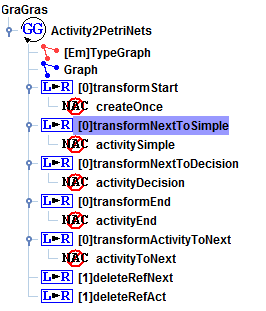
\includegraphics[scale=0.7]{figures/AGGTreeBasedEditor.png}
	\caption[Tree based editor in AGG]
	{Tree based editor for transformation rules.}
	\label{fig:AGGTreeBasedEditor}
\end{figure}

Whenever changes are made in the two graphs, AGG checks if the LHS or the RHS
conforms to the type graph. The user is unable to insert elements in the two
graphs that are not initialised in the type graph and the users are not allowed
by AGG to create associations between nodes that are not initialised in the type
graph. This is how AGG keep the source and target model consistent. In
figure~\ref{fig:AGGTreeBasedEditor} we can see the tree based editor in AGG,
that provides the type graph, the host graph and a list of application rules.
When a new application rule is created, both the LHS and the RHS of this new
rule is initialised. The users can then insert elements in both the LHS and the
RHS depending on how the source model should be translated. 

\begin{figure}[H]
	\centering
	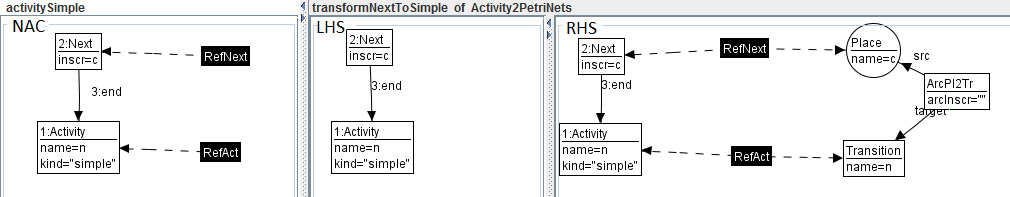
\includegraphics[scale=0.5]{figures/LHSvsRHSAGG.png}
	\caption[Representation of a rule in AGG]
	{The LHS and RHS of a rule and a NAC attached.}
	\label{fig:LHSvsRHSAGG}
\end{figure}

Figure~\ref{fig:LHSvsRHSAGG} is a representation of the rule
transformNextToSimple, with both the LHS and the RHS. Each rule can also
contain application conditions. These can either be Positive Application
Conditions (PAC) or Negative Application Conditions (NAC).
Figure~\ref{fig:LHSvsRHSAGG} has a NAC, activitySimple that makes sure that the
LHS of the rule is translated only once for each pattern match found in the
host graph. Through the use of these application conditions, the users can
create restrictions to how each transformation rule should handle pattern match
in the host graph. Each transformation rule can have multiple application
conditions attached.

\subsection{Administrating Transformation Rules}

By default, the control mechanism for administrating the transformation rules
are set to deterministically. This means that the transformation rules are
executed at random. This option is quite useful if the set of transformation
rules are independent of each other. AGG also provides other ways of applying
rules. These are transformation by applying rule layer or by sequences. When the
transformation is set to be applied by rule layers, then the user can add a
number to the different rules. This layer number will range from 0 \ldots n,
where the lowest number is the first layer and therefore the has first
priority. If there are many rules with the same layer number, then these rules
will be internally transformed deterministically. If the rules are applied
by sequence then the rules will be applied from the first element in the tree
based editor and applying the rest of the rules in sequence.

\subsection{Translating the Host Graph}

Now that we have defined the type graph and created the rules it is time to try
and translate the host graph. The preferred option on how the rules should be
applied has also been set. The user can now either press Start Transformation or
do the transformation one step at the time. When the user use the first option
AGG will apply one rule at the time until there is no more matches to be found.
When AGG cannot find any more matches, the host graph is either correctly
translated or there are errors in the rules. 

The user can also execute the transformation step by step. This will give the
user the same result as the first option, but now the user can do one match at
the time for each rule. 

\section{The Henshin Project}

The Henshin project\cite{Henshin} provides a model transformation
language and an editor for defining model transformations for the Eclipse
Modelling Framework \cite{Steinberg2009}. The Henshin project provides a
transformation language that has support for both endogenous and exogenous
model transformations and a provided graphical syntax. With the help of a
graphical editor, it provides the user with an intuitive way of representing
transformation rules. The Henshin Editor is build on the Eclipse Modelling
Framework and is integrated as an Eclipse plugin. The Henshin Editor was first
developed in a student project at Technical University of Berlin in 2010, and
extended in the bachelor thesis \cite{JohannSchmidt} of Johann Schmidt and the
master thesis \cite{AngelineWarning} of Angeline Warning.

\subsection{Graphical Editor}
Henshin model transformation language is a plugin for the Eclipse
Integrated Development Environment\cite{Eclipse}. The Henshin project provides
the users with a graphical editor to create and modify model to model
transformations. 

The users start out with using the Eclipse wizard to create an empty Henshin
document. The Henshin document is based on the commonly known Extensible Markup
Language (XML)\cite{XML}. If applicable a Henshin diagram file can be created
based on the Henshin file. This gives the users an intuitive approach to
creating model transformation rules.

The Henshin transformation file is represented in a tree based editor in
Eclipse called Henshin Model Editor. In this tree based editor it is possible
to include metamodels for both the source and the target model, represented in
figure~\ref{fig:Henshin_TreeEditor}. This figure represents the Henshin
Model Editor, where the different transformation rules for this case study is
presented. From this figure we can see that there is a Module element called
activity2Petrinets. This Module element will always be the root element for a
Henshin model transformation. This Module element contains all the user created
rules for performing a model transformation in Henshin. There is also two
external Ecore models included in the editor, more specifically the two
metamodels. These metamodels are created based on the EMF standard for creating
models and are independent of one and another.

\begin{figure}[H]
	\centering
	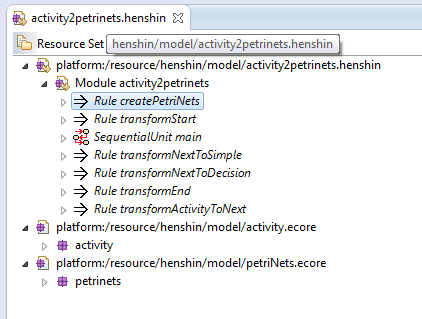
\includegraphics[scale=0.7]{figures/Henshin_TreeEdtiro.png}
	\caption[The Henshin Model Editor]
	{Tree Based Editor for rules in Henshin.}
	\label{fig:Henshin_TreeEditor}
\end{figure}

\subsection{Defining Metamodels}

The Henshin language requires a source and a target metamodel to be able to
perform model transformations. The target metamodel can either be the same as
the source metamodel or defined in another modelling language. Either way, before
the users can start creating transformation rules, the metamodels has
to be defined. To define these metamodels, Henshin use Ecore, that is
provided with the Eclipse Modeling Framework\cite{Steinberg2009}. Ecore models
can either be created using a tree based editor, called Sample Ecore Model
Editor or by using a graphical editor. While the graphical editor is optional,
the tree based editor is mandatory for creating Ecore models, since this is the
actual Ecore model. 

First the user has to create an EPackage element in the newly created Ecore
model. This EPackage is what Henshin searches for when the user want to import
an Ecore model. This EPackage element can have several child elements, like for
example EClass, EEnum and EData type. For our case study we only needed the
EClass element to create the nodes for the metamodels. And for each EClass
element the users can create EReference elements that can be connected with
other EClass elements. This means that an EReference element defines relations
between the nodes for the metamodels. To give an EClass element properties, the
user can create an EAttribute element. This element can be typed, either by a
predefined list of types or by defining user created EData types. For the
purpose of this case study we only needed to name the different nodes and
therefore we only needed the data type EString. Through the use of these Ecore
elements, we can create the two metamodels from
figure~\ref{fig:ActivityMetamodel} and figure~\ref{fig:PetriNetsMetamodel} from
problem specification in the first chapter.


\subsection{Defining Transformation Rules}

Now we have defined the source and target metamodel, and imported
both of the metamodels EPackages into the henshin model. We can now use elements
from the two metamodels to create transformation rules in the henshin model
language. In Henshin, objects are referred to as nodes and links between objects
as edges. From the metamodels these nodes represents the EClass elements and
edges is a EReference between these EClass elements. A collection of these nodes
and edges form a graph. This graph is what represent a transformation rule in
Henshin. It is also possible to define variables for each rule. These variables
can then be used to pass along attributes amongst nodes inside the
graph. 

Each transformation rule in Henshin will have two graph assigned.
These two graphs represent the LHS and the RHS of the rule. One thing that is worth mentioning is
that when working with the graphical editor, these graphs are unavailable for
the users to create or modify. Henshin handles assign the LHS and the RHS
through the use of stereotypes. Each rule can be represented as a graph in the
graphical editor. Figure~\ref{fig:HenshinScreen} is a visualization of the
graphical syntax of a specific transformation rule in Henshin.

\begin{figure}[H]
	\centering
	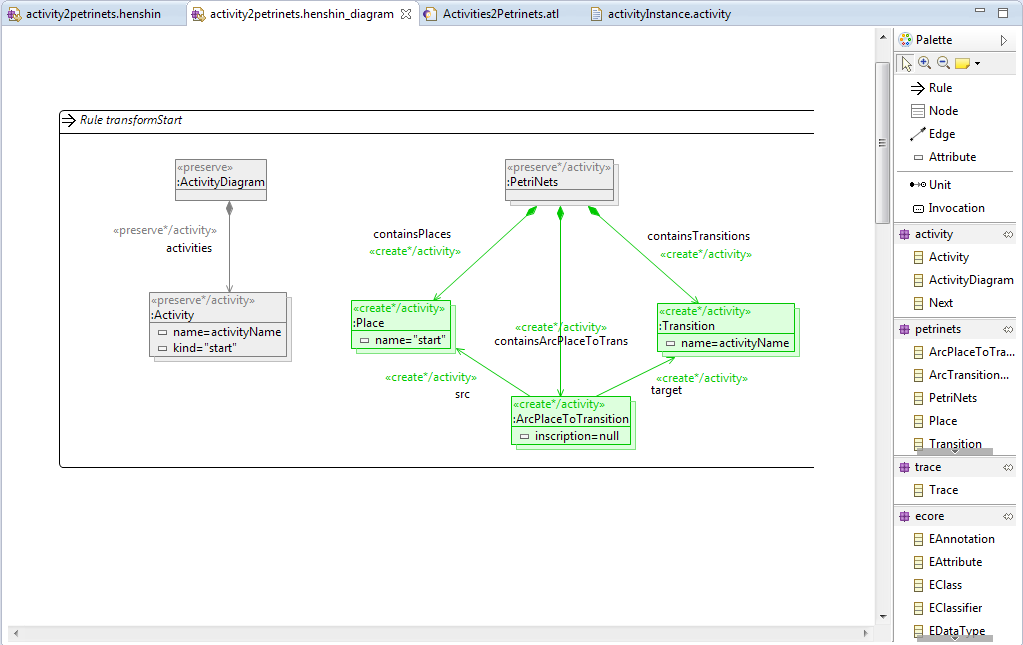
\includegraphics[scale=0.5]{figures/Henshin_Screen.png}
	\caption[The Henshin graphical editor]
	{A model transformation in the Henshin graphical editor}
	\label{fig:HenshinScreen}
\end{figure}

This rule is responsible for handling the start element for an activity.
On the right side there is a palette that contains Henshin elements and
different EPackages. The first two EPackages contains elements from the
metamodels we created. The next two EPackages are other models that can
be imported into Henshin. The Henshin Trace model is an EMF model that is used
to keep track of the translated elements during the transformation. This model
consist of a single class Trace, that has two references called source and
target. These references are of type EObject and therefore can refer to any EMF
object. This trace object can be used for all imported models used
in Henshin, since these models has to be defined from the Ecore model. Through
the use of the elements in the palette on right side of the window, the users
can create and modify elements. 
The Rule, Node, Edge and Attribute elements are used to define the different
transformation rules in Henshin. A new transformation rule in Henshin always
have to start with creating a new Rule element. Inside this Rule element the
users are free to create nodes, and connect these nodes with edges. At
all time Henshin makes sure that the created nodes and edges conform to their
corresponding models. The Attribute element can be used if attributes are
defined for the classes that are imported. The Unit element we will come back to
in the next section.

Henshin distinguish elements between the LHS and the RHS through the
use of predefined stereotypes, or action types. Henshin automatically delegates
these elements to the RHS or the LHS from these action types. If the action type
consist of the sequence <<create>>, Henshin knows that this element should be
part of the replacement graph, or the RHS. While on the other side, the sequence
<<delete>> should be part of the pattern graph, or the LHS. The <<preserve>>
sequence is a bit more special, because nodes or edges in Henshin that is of
this action type should be part of both the LHS graph and the RHS graph. This is
done by putting the preserve element in both graphs and then create a mapping
between these two elements to inform the Henshin Interpreter that this is the
same element.

Henshin also has support for application conditions. The action types <<forbid>>
and <<require>> are used for defining Negative Application Conditions (NACs)
and Positive Application Conditions (PACs). These actions are supported for
nodes, edges and attributes. Figure~\ref{fig:HenshinAction} is a representation
of how the users can choose amongst these action types.  

\begin{figure}[H]
	\centering
	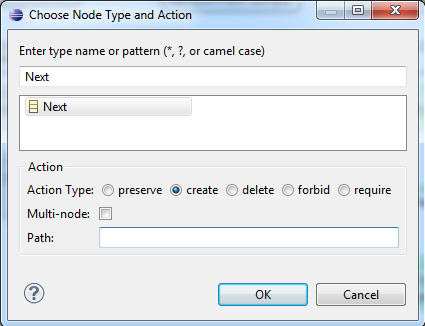
\includegraphics[scale=0.5]{figures/Henshin_Action.png}
	\caption[Action type for Henshin]
	{Action types for a Node.}
	\label{fig:HenshinAction}
\end{figure}

The ``Multi-node`` is a very special Henshin action type. This Henshin
feature gives the users the possibility to create nested multi-rules. This
concept used to be defined as an amalgamation unit in Henshin, but this feature
was changed to give users the opportunity to create rules inside rules. A
multi-rule action type would then be changed to <<create*>>, where the star
informs Henshin that this is a multi-rule. The Path option gives the users
the opportunity to give name this multi-rule. Multi-rule can be very useful if
there is a pattern in the instance graph that is matched more than once. The
users can then use this nested multi-rule concept to match and apply this rule
as often as possible.

\subsection{Transformation Units}
Transformation units in Henshin are used to administrate the different
transformation rules. There are several different units in Henshin that all have
different properties. It is important to mention that a rule is a unit,
since it inherits from a unit in the Henshin metamodel. This means that it is
unnecessary to create a unit in Henshin if our model transformation only
consist of one transformation rule. But if there are defined several
transformation rules there has to be a control mechanism that determines how
these transformation rules should be applied. A Independent Unit is a good
solution if the order of applying the transformation rules is not important.
But if the transformation rules follows a very strict pattern and are dependent
of other rules, then a sequential unit are a safe way to apply rules. The
sequential unit forces Henshin to apply rules in a given order.
Figure~\ref{fig:SequentialUnitHenshin} is an example of a sequential unit
that will start applying rules at the black circle and follow the arrow
through each given rule until it is finished.  

\begin{figure}[H]
	\centering
	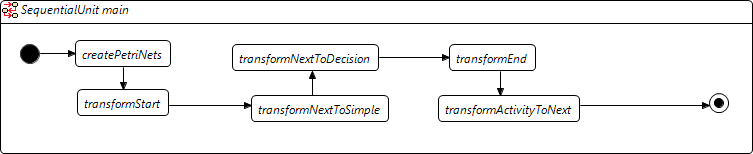
\includegraphics[scale=0.5]{figures/SequentialUnitHenshin.png}
	\caption[A Sequential Unit in Henshin]
	{A SequentialUnit main that contains a sequence of rules.}
	\label{fig:SequentialUnitHenshin}
\end{figure}

If applicable a transformation unit can also consist of other units, for example
if the user want to either iterate or loop through a transformation rules. This
can also be done with the use of a multi-rule, but in some cases this can only
be done by a LoopUnit or a IterateUnit. Henshin also has two other units that
can administrate transformation rules, namely ConditionalUnit and PriorityUnit.
The ConditionalUnit follows a if-else pattern, and is used if the user want
Henshin to choose between other units. 

\subsection{Translating the instance model}

Now that we have defined the source and target metamodel, created a set of
transformation rules and initialized a control mechanism for these rules it is
time to apply this transformation. For Henshin there is two ways to do this. In
Henshin the default engine for executing model transformation is the Henshin
interpreter. This interpreter can be invoked either by using the a Eclipse wizard
or programmatically using the Henshin API. 

Using the Eclipse wizard this is done by opening the Henshin file in the Henshin
Model Editor and right clicking the root object and locate apply transformation.
This will open a wizard where the user can choose a transformation unit. This
will either be a single transformation rule or some transformation unit that
applies all other units and rules. The user also has to select the instance
model and can explicitly set parameters for the rules if this is applicable. If
the parameter is set to Ignore then the interpreter will automatically match the
parameter. Now the user has two choices, the first choice is to preview the
result of the model transformation. This will either show the user a new window
with the modifications to the model or a message that the rule or unit could not
be applied. If the user press Transform instead of Preview, the model will be
transformed and saved.

The interpreter can also be invoked programmatically, either as an IApplication
in Eclipse or as a simple Java application. Henshin provides a API that lets the
users invoke the interpreter through the use of Java code. There is a class
HenshinResourceSet that lets the user load and save models and transformations.
When the instance model and Henshin module is loaded into the resource set, the
transformation can be applied through the use of the Henshin Engine class. This
is where Henshin finds and translates matches found in the instance graph. The
user also has to specify the main transformation unit from the Henshin module.
Both the engine and the unit can be loaded into the UnitApplication class. And
this class has a method called execute that lets the user execute the model
transformation. If the transformation was executed without errors, then the
instance model can be saved with the translated changes. The Henshin API lets
other users use the power of Henshin in their own program.

\section{ATL Transformation Language}

ATL\cite{ATL} (ATL Transformation Language) is a model transformation
language and is an answer to the QVT\cite{QVT} standard. It
provides ways to produce a set of target models from a set of source models.
ATL is developed on top of the Eclipse platform and is one of three
transformation engines provided by the Model to Model Transformation (MMT)
project\cite{MMT}. The MMT project hosts Model to Model Transformation
languages. These transformations are executed by transformation engines that are
plugged into the Eclipse Modeling infrastructure. MMT is a sub project of the
top level Eclipse Modeling Project\cite{EMP}. ATL is maintained by
OBEO\cite{OBEO} and AtlanMod\cite{ATLANMod} and was first initiated by the
AtlanMod team, previously called the ATLAS Group, located at the University of
Nantes in France. The initial version of ATL was created In 2004, where ATL
became part of the Eclipse Generative Modeling Technologies (GMT) \cite{GMT}.
The goal of GMT is to produce a set of research tools in the area of Model
Driven Software Development. The ATL Integrated Development Environment (IDE)
was later promoted for the Eclipse M2M project in January 2007.

\subsection{Textual editor}

ATL can be compared to a programming language, because it is
basically a transformation language. ATL is a text based transformation
language, and is build around the Object Constraint Language (OCL) \cite{OCL}
with some additional predefined functions. ATL transformations is stored in a
file extension called ``.atl'' These ATL files can contain different kind of
ATL units and are defined in its own distinct ATL file. These different ATL
units are ATL modules, ATL queries and ATL libraries. Libraries can be used to
create independent ATL libraries that can be imported to different types of ATL
units. The module unit specifies the different application rules for a  model
transformation. And the Queries are used when the users want to compute
primitive values from the source models.

Now that we have specified these three ATL units, we can describe shortly how
we can use the ATL transformation language to create model to model
transformations. For our case study, we only need the ATL modules. An ATL module
corresponds to a model to model transformation. This unit enables developers to
specify the way to produce a set of target models from a set of source models.
The source and target models of an ATL module must be consistent with their
respective metamodels. 

\subsection{Defining Metamodels}

Defining metamodels for the ATL language is defined by the modelling language
Ecore. Since defining the metamodels are defined the same way as Henshin, see
chapter 4.2.

At first, the user start out with a blank ATL file. Since we are working in
the ATL Integrated Development Environment for Eclipse, we want to start the
document with defining the path to the source and the target metamodel. The
reason for doing this is to achieve auto completion from elements defined in the
Ecore metamodels. This is convenient for the users when creating transformation
rules.  

\begin{figure}[H]
	\centering
	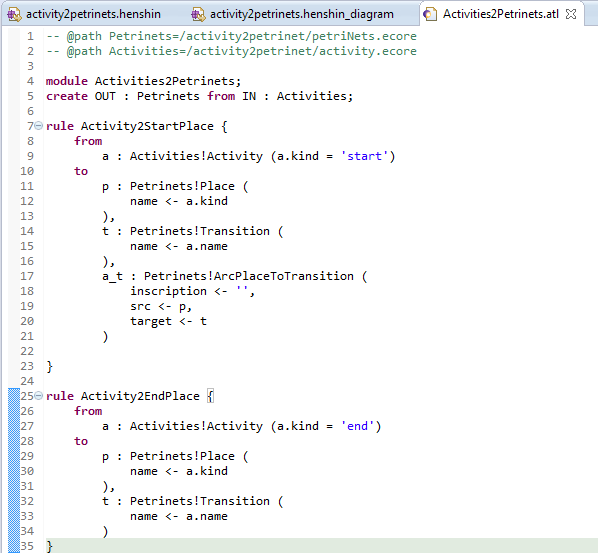
\includegraphics[scale=0.5]{figures/ATLScreen.png}
	\caption[ATL Textual Editor]
	{Two simple rules represented in ATL.}
	\label{fig:ATL_Screen}
\end{figure}

Next the file is composed of four different elements. The first element is the
header section, where the user can give the module a name and name the variables
corresponding from the source and target models. The module name has to be
identical to the name of the ATL file.

We also need to specify the source and the target metamodel. From
figure~\ref{fig:ATL_Screen} we can see that the target metamodel is initialised 
with the keyword create, and the source metamodel is initialised using the
keyword from. The user can also import some existing libraries if needed. This
import section is however optional. Importing metamodels are handled a bit
differently in ATL compared to Henshin. In ATL the metamodels are imported
explicitly while in Henhsin they are imported implicitly before they can be used
in modifying the transformation rules. For ATL the user has to configure where
both the source and the target metamodel are located through a configuration
page. 

\subsection{Defining Application Rules}

The next element is a set of rules that defines how the target models are
generated from the source models. These rules are used to implicitly match
source elements and produce target elements. In figure~\ref{fig:ATL_Screen} we
have examples of two rules, namely the rule for transforming the start activity
and the rule for transforming the end activity. We can see that for each rule we
specify what we want to translate from and what we want to translate to. 

The last element in a ATL module is a set of helper functions. This collection
of helpers can be compared to Java methods. These helper methods can be used to
make the transformation rules easier to read for example.

\subsection{Translating the instance model}

\begin{figure}[H]
	\centering
	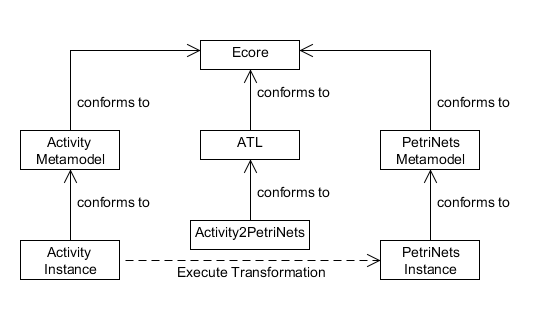
\includegraphics[scale=0.5]{figures/ATL.png}
	\caption[Model Transformation process for ATL]
	{Model transformation process for Activity2PetriNets.}
	\label{fig:ATL}
\end{figure}

Figure~\ref{fig:ATL} gives us an idea of how the ATL transformation from an activity
diagram to Petri net are handled. We want to generate a model PetriNets
instance, that conforms to the metamodel PetriNets. This is generated from a
source model, Activity Instance, that conforms to its respective metamodel.
The created transformation Activity2PetriNets is expressed in the ATL
transformation  language, that conforms to its own metamodel. These three
metamodels conform to the metamodel Ecore. So this makes Ecore a metametamodel
to represent the metamodels of Activity, ATL and PetriNets.

ATL has to be configured properly before the user can initiate a model
transformation. In this configuration both the location of the source and target
metamodel has to be specified. The user also has to specify what instance model
that should be translated. And lastly the user has to create a new file that can
be specified as the target instance model for the ATL run configuration. The
user can then initiate the transformation by running this as an ATL
transformation.
